\chapter{Introduction}
This document is intended to describe the main steps required for the integration and configuration of RTA-SUM Startup Shutdown Coordinator (SUSD).  
\ifnum \DocumentGroup=1
{General guidelines on the common steps and workflow for RTA-SUM integration can be found in \file{RTA-SUM Getting Started Guide}.}
\else
{%Nothing}
\fi

\section{Definitions and Abbreviations}
\input{generated/tables/definitions.tex}


\section{Module Overview}

\begin{figure}[htb]
\centering
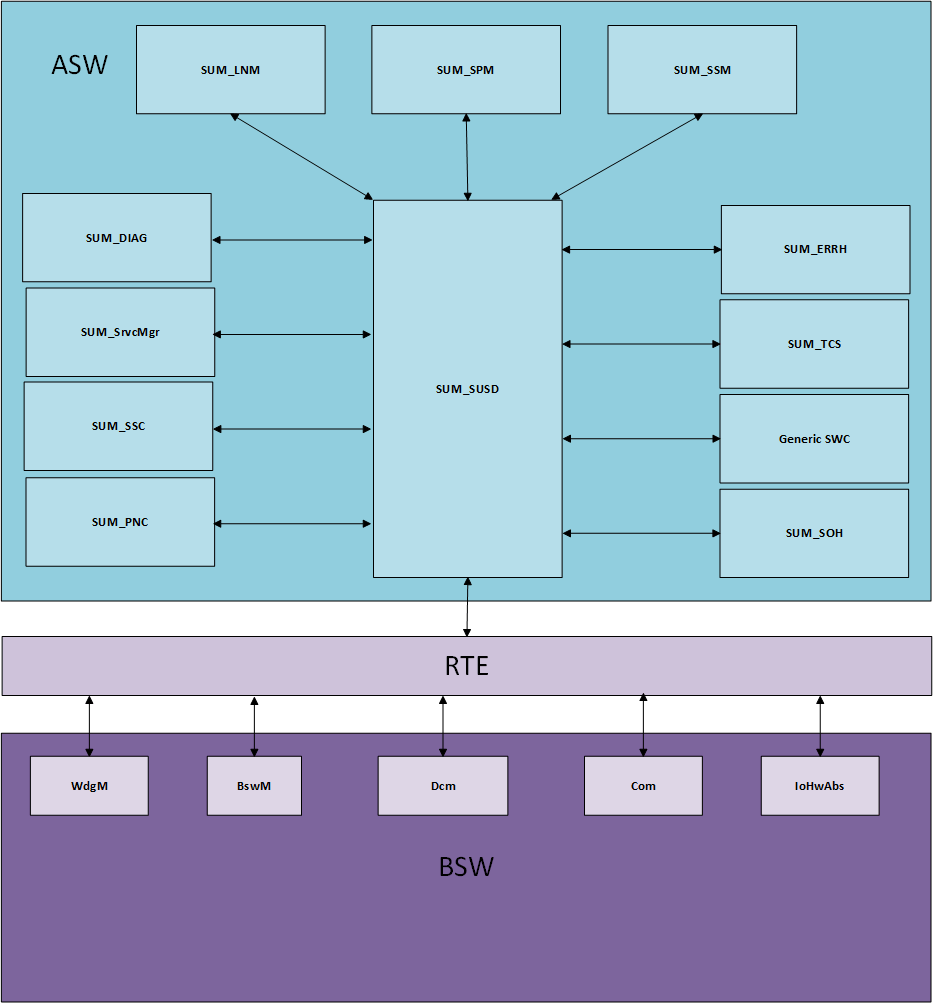
\includegraphics[width=0.5\textwidth]{images/layers.png}\caption{System layer overview.}\label{fig:layers}
\end{figure}

RTA-SUM SUSD is a software composition located in the Application Layer of the standardized architecture of AUTOSAR, as depicted in Figure \ref{fig:layers}. It implements the following functionalities:
\begin{itemize}
\item Application State Manager
\item Battery Voltage Monitor
\item Application Start / Shutdown
\item Run Crank Functionality
\item Power Moding Slave
\item Wakeup Related DIDs
\end{itemize}



\section{References}
\label{sec:ref}
\input{generated/tables/references.tex}

\section{User Guide Revision History}
\input{generated/tables/rev_history.tex}

